\chapter{FIFO Queue Algorithms and Analysis}
\label{Queue}

This chapter investigates different concurrent and transactional algorithms for queues to draw conclusions about concurrent queue algorithms in transactional settings. We begin with an overview of concurrent and transactional queue specifications and algorithms. We then evaluate how these queues perform on several microbenchmarks. Given our results, we conjecture that highly-concurrent queue algorithms are inherently unsuited to be converted for use as a fully transactional queue algorithm.

\section{Transactional Queue Specification}

A concurrent queue must adhere to the following specification, in which all operations can be ordered such that:
\begin{itemize}
    \item A value is popped off the queue only once (no duplicate pops).
    \item A value is pushed onto the queue only once (no duplicate pushes).
    \item Values are popped in the order in which they are pushed.
\end{itemize}

A transactional queue adds the following invariants to the specification. There must be a serial order of all transactions such that, within one transaction:
\begin{itemize}
    \item Any two pops pop consecutive values in the queue starting from the head of the queue .
    \item Any two pushes push consecutive values at the tail of the queue.
\end{itemize}

To satisfy these invariants, transactional data structures must support \emph{read-my-writes}. This is when a thread sees and modifies or returns the value from a previous operation in the transaction.


\emph{In the following discussion of our queue algorithms, we omit the discussion of the \texttt{front} operation to simplify reasoning about the state of the queue. An appropriate algorithm for \texttt{front} can be easily inferred from those used for pop.}

%%%%%%%%%%%%%%%%%%%%%%%%%%%%%%%%%%%%%%%%%%%%%%%%%%%%%%%%%%%%%%%%%%%%%%%%%%%%%%%%%%%%%%%%%%%%%%%%%%
\section{STO Queue Algorithms}

STO provides a transactional FIFO queue that adheres to the interface exposed by the \texttt
r{C++} standard library queue. The following transactional queue algorithms are designed with transactional correctness in mind, and concurrency as a secondary concern. 

The STO data type algorithms enforce transactional correctness using \emph{versions}. A version can act as a lock on the data structure: in order to update the data structure, a thread must first lock the version. A version also tracks changes to the data structure because it monotonically increases when a thread modifies the data structure. Thus, any version seen by a thread is equivalent to some previous or current state of the data structure. The first instance of the version observed by a thread during a transaction is checked when the transaction commits. This ensures that all observations are valid. Note that we cannot update the read version to an instance of the version observed later in the transaction. This is because we need to validate the first time we see the version in the transaction. 

\subsection{STO1 Queue}
The STO1 Queue is the first implementation of the transactional queue data structure using STO's framework. It implements a circular, fixed-size transactional queue.

The queue is implemented using optimistic concurrency control (OCC), which is a transactional algorithm that optimistically assumes that no other transaction will conflict with a thread's transaction. No thread prevents another thread from operating simultaneously on the queue during a transaction, which means multiple threads can add read/writes of the same parts of the queue during their transactions. Contention only occurs during commit time, when the thread must necessarily lock the queue so that it can safely verify and modify the queue's values without parallel modifications by other threads. A thread can only realize that another thread has “beaten” it to modifying the queue at commit time.

There are two versions for the queue that can potentially invalidate a transaction if either changes: a headversion, and a tailversion. The headversion tracks the location of the head of the queue, and the tailversion tracks the location of the tail of the queue.

The queue supports three transactional operations: push, pop, and \texttt{front}. A push within a transaction adds to an internal \texttt{write\_list\_item}. This \texttt{write\_list} holds thread-local list of values to be pushed onto the queue, which are added to the tail of the queue during commit time (ensuring all values are added consecutively). We observe that all transactions comprised of only pushes will always commit because pushes do not observe any property of the queue: one transaction's pushes and pops do not affect the outcome of another's pushes. (Note, however, that the opposite is not true). During commit time, the thread locks the tailversion so that no other thread's push can push onto the queue. The items on the \texttt{write\_list} are added to the queue, and the tailversion incremented.

A pop within a transaction first checks if the queue is empty. If the queue is empty, then the thread reads the tailversion to ensure that no other transaction has committed a push before this thread commits. Suppose another thread successfully installs a push before this thread commits. Then this pop should have read that pushed value instead of seeing an empty queue. This forces the thread to abort the transaction. If there have been items added to the \texttt{write\_list} from previous pushes within the transaction, then the pop will “pop” an item off the \texttt{write\_list}, performing an instance of \emph{read-my-writes}. Such a modiicatio is allowable during execution time because the \texttt{write\_list} is thread-local. If the queue is nonempty, then the thread reads the headversion to ensure that no other transaction has committed a pop before this thread commits. The thread then finds the item to pop off the queue by iterating through the queue from the head until it finds an item that has not yet been popped off within this transaction. The thread adds a write to this item so it knows during commit time and during future pops that it intends to pop this item.

The design is summarized in Table \ref{table:sto1}.

\subsection{STO2 Queue}
The STO2 Queue is also a circular, fixed-size queue, with operations push, pop, and front. The STO2 Queue algorithm is a hybrid design integrating the STO1 algorithm with another transactional algorithm: pessimistic locking. This takes inspiration from the transactional queue from the Transactional Data Structures Library\cite{TDSL} as described in previous work. Their pessimistic transactional queue appears to achieve better performance in their benchmarks than the STO1 queue, and the algorithm is simpler to implement and describe. 

Pessimistic locking entails locking the queue when any naturally-contentious operation (e.g., pop) is invoked. The queue is then only unlocked after the transaction is complete. This ensures that no other thread will execute an operation that may invalidate a pop within this thread's transaction. However, operations such as ``push'' that can operate without any wait do not require locking during execution. Therefore, a push follows the same protocol as in the STO1 queue.

Because pop locks the queue, there are no conflicts at commit time. A thread only aborts if it fails to obtain the lock after a bounded period of time. The one version, “queueversion,” acts as the global queuelock. 

The design is summarized in Table \ref{table:sto2}

%%%%%%%%%%%%%%%%%%%%%%%%%%%%%%%%%%%%%%%%%%%%%%%%%%%%%%%%%%%%%%%%%%%%%%%%%%%%%%%%%%%%%%%%%%%%%%%%%%

\section{Flat Combining Queue Algorithms}
Given the relatively slow performance of our STO queues, we looked to find a highly-concurrent (non-transactional) queue algorithm that would be promising to integrate with STO's transactional framework. After running several benchmarks (see Figure \ref{fig:concurrent_queues}), we found the most promising to be the Flat-Combining technique, which not only outperforms other queue algorithms, but also addresses several of the bottlenecks we observe in the STO queues.

\subsection{Flat Combining Queue (Non-Transactional)}
\label{fcqueuent}


Flat Combining, proposed by Hendler, et. al. in 2010\cite{flatcombining}, is a synchronization technique that is based upon coarse-grained locking and single-thread access to the data structure. The key insight is that the cost of synchronization for certain classes of data structures often outweighs the benefits gained from parallelizing access to the data structure. These data structures include high-contention data structures such as stacks, queues, and priority queues. Created with this insight, the flat combining algorithm proposes a simple, thread-local synchronization technique that allows only one thread to ever access the data structure at once. This both reduces synchronization overhead on points of contention (such as the head of the queue) and achieves better cache performance by leveraging the single-threaded access patterns during data structure design.

The data structure design includes a sequential implementation of the data structure, a global lock, and per-thread records that are linked together in a global publication list. A record allows a thread to publish to other threads the specifics of any operation it wants to perform; the result of the operation is subsequently written to and retrieved from the record.

When a thread T wishes to do an operation O:
\begin{enumerate}
    \item T writes the opcode and parameters for O to its local record. Specifically for the queue, the thread writes \texttt{<PUSH, value>} or \texttt{<POP, 0>} to its local record.
   \item T tries to acquire the global lock.
   \begin{enumerate}
        \item T acquires the lock and is now the “combiner” thread. T applies all thread requests in the publication list to the data structure in sequence, and writes both the result and an \texttt{<OK>} response to each requesting thread's local record.
        \item T failed to acquire the lock. T spins on its record until another thread has written the result to T's record with the response \texttt{<OK>}.
    \end{enumerate}
\end{enumerate}

In the context of the queue, flat combining proves to be an effective technique to handle the contention caused by parallel access on the head and tail of the queue. In addition, their choice of queue implementation uses ``fat nodes'' (arrays of values, with new nodes allocated when the array fills up), which both improves cache performance and allows the queue to be dynamically sized. Both the STO1 and STO2 queues suffer from the contention and cache performance issues pointed out in the flat combining paper, leading us to believe that flat combining's alternative synchronization paradigm might improve the performance of a transactional queue as much as it does for a concurrent queue.

\subsection{Flat Combining Queue (Transactional)}
\label{fcqueuet}

Recall that, in addition to the requirements for a correct concurrent queue, a transaction queue must guarantee that there must be a serial order of all transactions such that, within one transaction, any two pops pop consecutive values in the queue starting from the head of the queue and any two pushes push consecutive values at the tail of the queue.

In order to add transactional guarantees to the flat combining queue, the order in which threads' requests are applied to the queue becomes important. For example, let a transaction in thread T1 be \texttt{pop, pop} and a transaction in thread T2 be pop. The combiner thread sees \texttt{T1:pop} and \texttt{T2:pop}, and applies both operations to the queue. T1 second pop request will violate the transactional specification because the two popped values in T1's transaction will not be consecutive. T1 must now abort, which means T2's pop is now invalid: it does not represent a pop at the head of the queue.

Addressing the scenario described above requires two important changes to flat combining (we describe the rational for these changes in Chapter~\ref{commutativity}): 
\begin{enumerate}
\item pushes cannot be applied to the queue during a transaction's execution, and must instead be performed when a transaction commits
\item An uncommitted pop in a thread's transaction must be unobservable by any other thread. This can be implemented in two ways:  
    \begin{enumerate}
        \item The algorithm can delay a transaction's pops until commit time. This algorithm must track which values in the queue are going to be popped within the transaction. This prevents duplicate pops and detects if the queue will be ``empty'' given how values will be popped.
        \item The algorithm does not execute flat combining requests from other threads until the transaction has committed or aborted. This can be implemented either through making other threads' transactions abort, or by causing the threads to block or spin.
    \end{enumerate}
\end{enumerate}

We now describe the new algorithms for push and pop.  We change the types of request a thread can publish to its record on the publication list. Recall that the original flat combining queue supports two requests: \texttt{<PUSH, value>} and \texttt{<POP, 0>}. The transactional queue supports the follow requests:
\begin{itemize}
    \item \texttt{<PUSH, list>} : push a list of values onto the queue
    \item \texttt{<MARK\_POP, thread\_id>} : mark a value in the queue to be popped by this \texttt{thread\_id}
    \item \texttt{<DEQ, thread\_id>} : dequeue all values in the queue that are marked by this \texttt{thread\_id}
    \item \texttt{<EMPTY?, thread\_id>} : check if the queue, after popping all items marked by this \texttt{thread\_id}, is empty
    \item \texttt{<CLEANUP, thread\_id>} : unmark all values that are marked with this \texttt{thread\_id}
\end{itemize}

As with the STO1 queue, a push within a transaction adds to an internal \texttt{write\_list\_item}. At commit time, the thread will invoke the \texttt{<PUSH, list>}, with the \texttt{write\_list} passed as the argument.

A pop is implemented with a pessimistic approach. Performing a pop within a transaction invokes the \texttt{<MARK\_POP, thread\_id>} command. The combiner thread, upon seeing a MARK\_POP command, looks at the first value at the head of the queue. If this value is marked with another thread's \texttt{thread\_id}, the combiner thread returns \texttt{<ABORT>} to the calling thread.

If the value is not marked, the combiner thread marks the value with the caller's \texttt{thread\_id} and returns \texttt{<OK>}. Else the value is marked by the calling thread's \texttt{thread\_id}. Note that in this scenario, no other thread can have marked values in the queue, since they will abort when seeing the head value marked by the calling thread's \texttt{thread\_id}. The combiner thread iterates sequentially through the queue values until it reaches a value not marked by the calling thread's \texttt{thread\_id}. It then marks the value with the caller's \texttt{thread\_id} and returns \texttt{<OK>}. Upon receiving the response, the calling thread adds a write to a \texttt{pop\_item} to tell the thread to post a \texttt{<DEQ, thread\_id>} request at commit time. This removes the popped value from the queue.

If the queue is either empty or there are no values not marked with the caller's \texttt{thread\_id}, the combiner thread will return \texttt{<EMPTY>}, which is remembered by the calling thread. An \texttt{<EMPTY>} response requires that the size of the queue be checked at commit time.

Note that this algorithm does not allow pops to read the values pushed within the same transaction. To do so would require passing in the thread's \texttt{write\_list} in addition to the \texttt{thread\_id} as arguments to the combiner thread. During our evaluation, we leave this part of the transactional queue specification unimplemented (and expect that adding this will only decrease performance).

The \texttt{<EMPTY?, thread\_id>} request is posted when a thread attempts to commit a transaction that observed an empty queue at some point in its execution. This happens when the thread receives an \texttt{<EMPTY>} response to a \texttt{<MARK\_POP>} request during the transaction. If the response to \texttt{<EMPTY?>} is true, then the thread knows that no other thread has pushed onto the queue between the time of its \texttt{<MARK\_POP>} seeing an empty queue and commit time. Else another thread has pushed items onto the queue, invalidating this thread's pop result, and this thread must abort.

If a thread ever sees an empty queue when executing a pop \emph{and} subsequently performs a push within the same transaction, the thread must prevent another transaction from committing between the time of the empty check and the installation of its pushed value. This requires adding what is essentially a lock of the tail of the queue. This is implemented via additional machinery in the combiner thread, which signals whether or not a transaction has locked the queue, and prevents any other thread's pushes from being installed until the ``lock'' is released.\lyt{TODO ACTUALLY IMPLEMENT}

The \texttt{<CLEANUP, thread\_id>} request is posted when a thread aborts a transaction and must unmark any items in the queue that it had marked as pending pops. The combiner thread iterates through the queue from the head and unmarks any items with the \texttt{thread\_id}.

The algorithm is summarized in Table \ref{table:fcqueue}.

\begin{table}[ht!]
    \scriptsize
\centering
\begin{tabular}{|c|c|c|c|c|l|}
\hline
    \multicolumn{2}{|c|}{Operation} & Execution-Time Effects & Read Set & Write Set & \multicolumn{1}{c|}{Commit Protocol} \\ 
    \hline\hline
    \multicolumn{2}{|c|}{Push} & none & none & \texttt{write\_list}& 
        \begin{tabular}[c]{@{}l@{}}- lock tailversion\\ - perform pushes\\ - increment tailversion\\ - unlock tailversion\end{tabular}\\ 
    \hline
    \multirow{2}{*}{Pop} & Nonempty & none & headversion & element to be popped & \begin{tabular}[c]{@{}l@{}}- lock headversion\\ - check headversion\\ - perform pops\\ - increment headversion\\ - unlock headversion\end{tabular} \\
    \cline{2-6} 
                     & Empty & none & tailversion & none  & 
                     \begin{tabular}[c]{@{}l@{}}- lock tailversion\\ - check tailversion\\ - unlock tailversion\end{tabular} \\
\hline
\end{tabular}
\caption{The STO1 Queue Algorithm}
\label{table:sto1}
\end{table}

%%%%%%%%%%%%%%%%%%%%%%%%%%%%%%%%%%%%%%%%%%%%%%%%%%%%%%%%%%%%

\begin{table}[ht!]
    \scriptsize
\centering
    \begin{tabular}{|c|c|c|c|c|l|}
\hline
    \multicolumn{2}{|c|}{Operation} & Execution-Time Effects & Read Set & Write Set & \multicolumn{1}{c|}{Commit Protocol} \\ 
    \hline\hline
    \multicolumn{2}{|c|}{Push} & none & none & \texttt{write\_list}& 
        \begin{tabular}[c]{@{}l@{}}- lock queueversion,\\ - perform pushes,\\ - increment queueversion\\ - unlock queueversion\end{tabular}\\ 
    \hline
    \multirow{2}{*}{Pop} & Nonempty & lock queueversion & none & element to be popped  & \begin{tabular}[c]{@{}l@{}}- perform pops\\ - unlock queueversion\end{tabular} \\
    \cline{2-6} 
                     & Empty & lock queueversion & none & none & none\\
\hline
\end{tabular}
    \caption{The STO2 Queue Algorithm (delayed pop execution)}
\label{table:sto2}
\end{table}

%%%%%%%%%%%%%%%%%%%%%%%%%%%%%%%%%%%%%%%%%%%%%%%%%%%%%%%%%%%%
\begin{table}[ht!]
    \scriptsize
\centering
    \begin{tabular}{|c|c|c|c|c|l|}
\hline
    \multicolumn{2}{|c|}{Operation} & Execution-Time Effects & Read Set & Write Set & \multicolumn{1}{c|}{Commit Protocol} \\ 
    \hline\hline
        \multicolumn{2}{|c|}{Push} & none & none & \texttt{write\_list}& \texttt{<PUSH, write\_list>}\\
    \hline
        \multirow{2}{*}{Pop} 
                     & Nonempty & \texttt{<MARK\_POP, thread\_id>} & none & \texttt{pop\_item} & \texttt{<DEQ, thread\_id>}\\
    \cline{2-6} 
                     & Empty & none & none & \texttt{pop\_item} & check \texttt{<EMPTY?, thread\_id>}\\
\hline
\end{tabular}
    \caption{The Transactional Flat Combining Queue Algorithm (delayed pop execution)}
\label{table:fcqueue}
\end{table}

%%%%%%%%%%%%%%%%%%%%%%%%%%%%%%%%%%%%%%%%%%%%%%%%%%%%%%%%%%%%
\iffalse
\begin{table}[ht!]
    \scriptsize
\centering
    \begin{tabular}{|c|c|c|c|c|l|}
\hline
    \multicolumn{2}{|c|}{Operation} & Execution-Time Effects & Read Set & Write Set & \multicolumn{1}{c|}{Commit Protocol} \\ 
    \hline\hline
    \multicolumn{2}{|c|}{Push} & none & none & \texttt{write\_list}& 
        \begin{tabular}[c]{@{}l@{}}- lock queueversion,\\ - perform pushes,\\ - increment queueversion\\ - unlock queueversion\end{tabular}\\ 
    \hline
    \multirow{2}{*}{Pop} & Nonempty & lock queueversion, perform pop & none & element to be popped  & unlock queueversion \\
    \cline{2-6} 
                     & Empty & lock queueversion & none & none & none\\
\hline
\end{tabular}
    \caption{The STO2 Queue Algorithm (undo logging)}
\label{table:sto2pops}
\end{table}
\fi


\section{Evaluation}

\subsection{Microbenchmarks}
\label{q_microbenchmarks}

All queues are evaluated on a set of microbenchmarks to demonstrate their scalability and performance. The controlled nature of these microbenchmarks allow us to easily compare particular aspects of each algorithm, such as transactional overhead introduced by STO. All experiments are run on a 100GB DRAM machine with two 6-core Intel Xeon X5690 processors clocked at 3.47GHz. Hyperthreading is enabled in each processor, resulting in 24 available logical cores. The machine runs a 64-bit Linux 3.2.0 operating system, and all benchmarks and STO data structures are compiled with g++-5.3. In all graphs, we show the median of 5 consecutive runs with the minimum and maximum performance results represented as error bars.\lyt{TODO}

\subsubsection{Parameters}

\begin{itemize}
\item Value Types: Each queue benchmark uses randomly chosen integers. This is because the benchmark tests do not manipulate the values they push/pop and the queue algorithms are agnostic to the actual values being placed in the queue.

\item Initial Queue Size: We run several tests with different initial fullness of the data structure. This affects how often the structure becomes empty, which can cause aborts and additional overhead (as described in the algorithms above). It also affects the number of cache lines accessed: a near-empty queue will never require iterating over values contained in more than one cache line.

\item Transaction Size: We modify the number of operations per transaction in different benchmarks. For some benchmarks, the number of operations in a transaction is set to 1 (i.e., the transactions are singleton transactions). This provides a more fair evaluation of transactional data strucures against concurrent data structures: by keeping a transaction as short as possible, we minimize the performance hit from transactional overhead. In order to support multiple-operation transactions, STO adds overhead which includes support for multiple items in read/write sets, read-my-writes, and an increased number of aborts and retries. With single operation transactions, we observe an upper bound on the best performance our data structures can achieve.

\item Data Structure Opacity: If opacity is enabled, a transaction will abort immediately if any inconsistent state is detected. This requires keeping track of a global transaction ID (TID). This global TID must be accessed when a transaction commits and when items are added to the read set during a transaction's, making transactions overall more expensive. For our benchmarks, we consider only queues without opacity enabled (as to measure its maximum achievable performance).\lyt{do we need this?}
\end{itemize}

\subsubsection{Tests}
\begin{enumerate}
\item 2-Thread Push-Pop Test: This test has one thread that performs only pushes and another thread that performs only \texttt{pops}. Unless the queue is empty, the two threads should never be modifying the same part of the data structure, and will never conflict (abort rate should be near 0). We use this test to measure the speed of push/pops on the queue when contention is not an issue. We expect that our transactional queues should perform as well, if not better, than most of the high-concurrency queues: while their algorithms are optimized for multi-threaded access, our simpler implementation should be just as fast with low contention and low abort rates.

\item Multi-Thread Singletons Test: 
    In this test, a thread randomly selects an operation (push or pop) to perform within each transaction. This keeps the queue at approximately the same size as its initial size during the test. This test is run with different initial queue sizes and different numbers of threads, which each thread performing singleton transactions. This test allows us to benchmark performance under variable amounts of contention (by increasing the number of threads) and increased abort rates. We expect that our STO1/STO2 transactional queues will perform significantly worse once the number of threads is increased and our naive concurrency algorithms underperform concurrency algorithms optimized for contentious situations.
    
%\item Multi-Thread Random Multi-Operation Transactions Test: 
    %In this test, a thread randomly selects multiple operations (push or pop) to perform within each transaction. This keeps the queue at approximately the same size as its initial size during the test. This test is run with different initial queue sizes and different numbers of threads. This test is most useful to compare different transactional data structures.
    
\end{enumerate}

\subsection{Results}

We describe the results of these benchmarks for two sets of queues. The first is a set of high-concurrency, non-transactional queues, and the second is a set of variations of the flat-combining queue (transactional and non-transactional). Both sets are measured along with our STO1 and STO2 queues as baseline references.

\subsubsection{Concurrent Queues}

We benchmark a set of the best-performing high-concurrency queue algorithms against our two STO queue implementations in order to determine which high-concurrency algorithm would be best suited to integration with STO. We look for both the most scalable and the highest-performing queue (even when contention is low).
 
 Our implementation of the flat combining queue modifies the implementation of the flat combining queue from the authors of the flat combining paper\cite{flatcombining}. Our implementation of the other high-concurrency queues are taken from the Concurrent Data Structures (CDS) library implementations online\cite{libcds}. The performance of these implementations on our tests the performance results given in the papers that originally proposed the algorithms.\lyt{CHECK}


\paragraph{2-Thread Push-Pop Test}
\begin{figure}[ht!]
\centering
    \includegraphics[height=3in]{concurrent/Q:PushPopspeed.png}
\caption{2-Thread Push-Pop Test Results of Various Concurrent Queues}
\label{fig:concurrent_queues}
\end{figure}

\paragraph{Multi-Thread Random Singleton Transactions Test}
\begin{figure}[ht!]
\centering
    \begin{minipage}{0.45\textwidth}
        \centering
        \includegraphics[height=2.5in]{concurrent/Q:RandSingleOps10000speed.png}
        \caption*{Initial Queue Size of 10000.\\Performance (ops/s) (higher is better)}
    \end{minipage}
    \begin{minipage}{0.45\textwidth}
        \centering
        \includegraphics[height=2.5in]{concurrent/Q:RandSingleOps100000speed.png}
        \caption*{Initial Queue Size of 100000.\\Performance (ops/s) (higher is better)}
    \end{minipage}
\caption{Multi-Thread Singletons Test Results of Various Flat-Combining and Transactional Queues}
\label{fig:concurrent_queues}
\end{figure}

Out of the concurrent data structures tested, the read-write queue\cite{queue1} and the flat combining queue consistently perform best on the 2-Thread Push-Pop Test. On the Multi-Thread Random Singleton Test, the flat combining queue achieves performance over $2.5\times$ greater than any other queue as the number of threads increases above 2.

For these reasons, as well as the algorithmic benefits of the flat combining technique described in Section~\ref{fcqueuent}, we focus our work on the flat combining queue.

We include the STO1 and STO2 queues in these benchmarks to measure the signficance of the gap between transactional and concurrent data structures. The STO queues---particularly the STO2 queue---outperform all but the read-write queue and flat combining queues on the 2-thread Push-Pop test. This test incurs the least contention and transactional overhead to track simply how fast the data structure can handle pushes and pops. It is unsurprising that, on this test, a simple synchronization strategy, such as that used in the STO queues, outperforms the majority of high-concurrency algorithms which are optimized for scalability. The Multi-Thread Random Singleton Transaction test demonstrate that as contention and transactional overhead (abort rate) increases, the flat combining queue maintains performance approximately 2.5$\times$ greater than that of the STO queues, although neither algorithm scales. However, the other high-concurrency algorithms appear to perform worse than our STO queues. We conjecture this may be due to the implementation of the algorithm used in our benchmarks\cite{libcds}.

\subsubsection{Flat Combining Queue Variants}

We benchmark several variants of the flat combining queue against our STO1 and STO2 queues. This includes:
\begin{itemize}
    \item FCQueueNT: the non-transactional flat combining queue.
    \item STO-FCQueue: the fully-transactional flat-combining queue.
    \item WrappedFCQueueNT: the non-transactional flat combining queue that invokes STO \texttt{start\_transaction} and \texttt{commit\_transaction} calls, but does not do any of the transactional bookkeeping necessary to provide transactional guarantees.
\end{itemize}

The relative performance of the WrappedFCQueueNT to the FCQueueNT indicates how much of the overhead added by the STO system is unavoidable (without modifications to STO itself). A data structure must always invoke the STO wrapper calls to support transactions. 

\paragraph{2-Thread Push-Pop Test}
\begin{figure}[ht!]
    \centering
    \begin{minipage}{0.45\textwidth}
    \centering
    \includegraphics[height=2in]{fcqueues/Q:PushPopspeed.png}
    \caption*{Performance (ops/s)\\(higher is better)}
    \end{minipage}
    \begin{minipage}{0.45\textwidth}
    \centering
    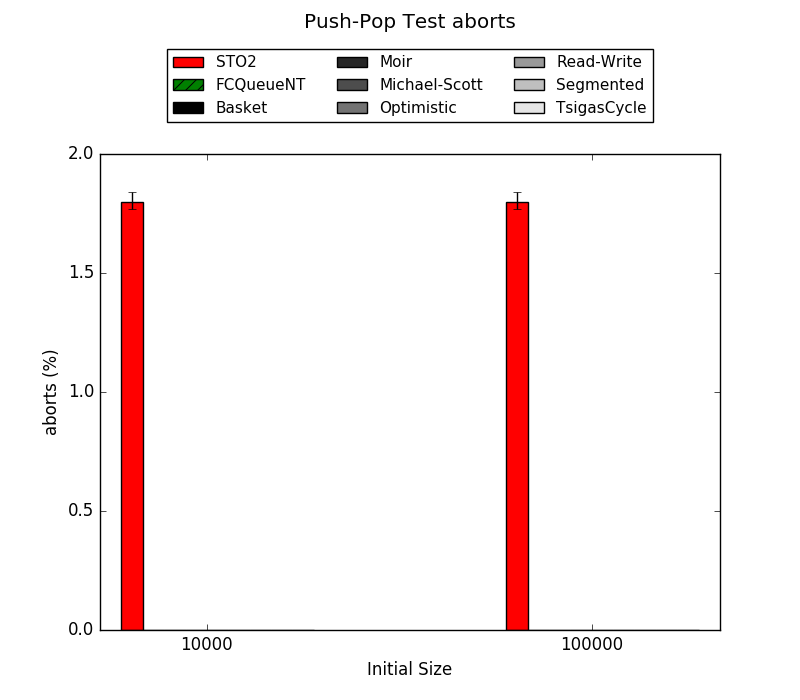
\includegraphics[height=2in]{fcqueues/Q:PushPopaborts.png}
    \caption*{\%Aborts\\(lower is better)}
    \end{minipage}
\caption{2-Thread Push-Pop Test Results of Various Flat-Combining and Transactional Queues}
\label{fig:fcqueues_queues}
\end{figure}

\paragraph{Multi-Thread Singletons Test}
\begin{figure}[ht!]
    \centering
    \begin{minipage}{0.45\textwidth}
    \centering
    \includegraphics[height=2.5in]{fcqueues/Q:RandSingleOps10000speed.png}
    \caption*{Initial Queue Size of 10000.\\Performance (ops/s) (higher is better)}
    \end{minipage}
    \begin{minipage}{0.45\textwidth}
    \centering
    \includegraphics[height=2.5in]{fcqueues/Q:RandSingleOps100000speed.png}
    \caption*{Initial Queue Size of 100000.\\Performance (ops/s) (higher is better)}
    \end{minipage}
    \\
    \begin{minipage}{0.45\textwidth}
    \centering
    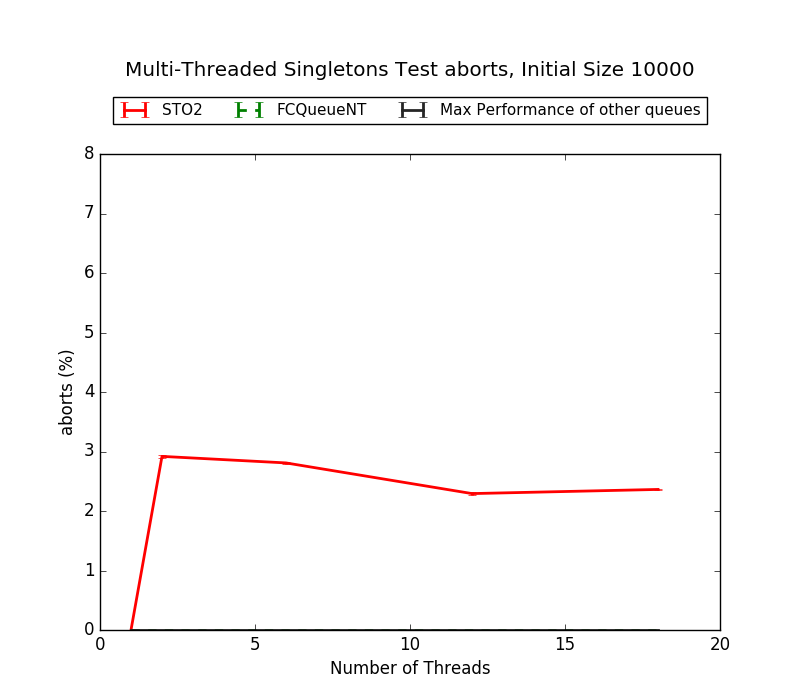
\includegraphics[height=2.5in]{fcqueues/Q:RandSingleOps10000aborts.png}
    \caption*{Initial Queue Size of 10000.\\\%Aborts (lower is better)}
    \end{minipage}
    \begin{minipage}{0.45\textwidth}
    \centering
    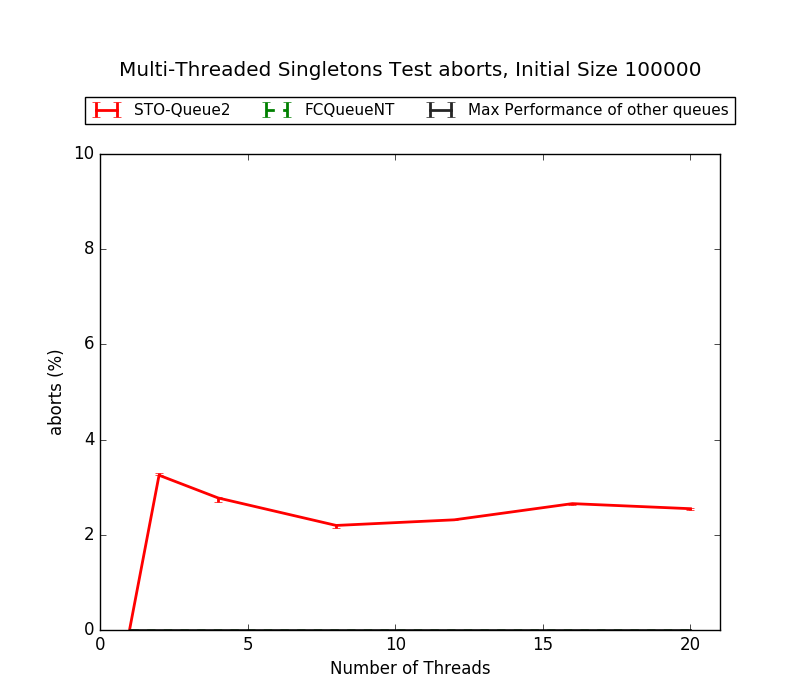
\includegraphics[height=2.5in]{fcqueues/Q:RandSingleOps100000aborts.png}
    \caption*{Initial Queue Size of 100000.\\\%Aborts (lower is better)}
    \end{minipage}
\caption{Multi-Thread Singletons Test Results of Various Flat-Combining and Transactional Queues}
\label{fig:txnal_queues}
\end{figure}


\section{Discussion}

\subsection{STO Overhead}
We first analyze what our results tell us about STO itself. Benchmarking transactional queues with naive concurrency algorithms (STO1 and STO2) against various high-concurrency algorithms demonstrates a simple implementation of a naive algorithm can consistently outperform more complex concurrent queue implementations even given the additional STO overhead. This indicates that the overhead added from STO does not cripple performance if used carefully---our transactional data structures can compete with several high-concurrency, non-transactional data structures. However, we see by comparing to the non-transactional flat combining queue that our algorithms are certainly not optimal for performance in a non-transactional setting.

Our comparison of the WrappedFCQueueNT and the FCQueueNT demonstrates that STO introduces some signficant necessary overhead \lyt{actual numbers here}. The STO wrapper calls (\texttt{start\_transaction} and \texttt{commit\_transaction}) allow a thread to mark which operations should occur together in the same transaction. After invoking the \texttt{start\_transaction} call, the thread can collect items in its read- and write-set; when \texttt{commit\_transaction} is invoked, the commit procedure is run (validation and installation of items in the read-/write-sets). The WrappedFCQueueNT adds no items to the read-/write-sets after invoking \texttt{start\_transaction}, and therefore incurs the minimum amount of overhead necessary to use STO:\ the commit procedure has zero items to validate or install. The WrappedFCQueueNT therefore represents the upper bound of performance we can expect from our STO queues. Even with the wraper calls, our results indicate it can still be possible to achieve performance \lyt{numbers} times greater than that of our original STO1 and STO2 queues.

\subsection{Transactional Flat Combining Queue}

Our results for the flat combining queue variants indicate that the fully-transactional flat combining queue algorithm (STO-FCQueue) performs poorly. Analysis with the \texttt{perf} tool indicates that the majority of the overhead is incurred from spinning on the flat combining lock (acquired by the combiner thread) or waiting for a flat combining call to complete. We see these results because of two reasons:
\begin{enumerate}
\item \emph{Higher Quantity}: A thread must make multiple flat combining calls to perform a pop within a transaction (recall that a push only requires one flat combining call) 
\item \emph{Higher Complexity}: each flat combining call requires executing instructions, which makes each operation request more expensive.
\end{enumerate}

We conclude that the flat combining technique, while perhaps near-optimal for a highly-concurrent data structure, is no better in a transactional setting than a naive synchronization technique such as that used in the STO1 and STO2 queues. This is because the flat combining algorithm must track the transaction state (e.g., going to perform two pops, one of which observes an empty queue) in order to provide transactional guarantees. In the next chapter, we formalize this argument using a commutativity discussion and claim that the higher quantity of more complex flat combining calls is necessary for flat combining to be used in a transactional setting: the flat combining technique depends on operation commutativity present in only a non-transactional setting to achieve its high performance. 

